\documentclass{article}
\usepackage{graphicx}

\title{Labwork 3: Gray Image}
\author{Nguyen Nhu Duy}
\date{}

\begin{document}

\maketitle

\section{Implementation}

An RGB image of size $6000 \times 3375$ was loaded and reshaped into
$20,250,000 \times 3$ RGB values. Grayscale conversion was implemented
using a CPU for-loop and a Numba CUDA kernel. Execution time was measured using \texttt{time.time()}.

The CPU execution time was 23.618 s and the GPU execution time was
0.0274 s, giving a speedup of approximately $862.16\times$.

\section{Block Size Experiment}

Different CUDA block sizes from 8 to 512 were tested. The execution time decreased from 0.0425 s to around 0.028 s. 
The fastest execution time was 0.02788 s with a block size of 256. Increasing the block size improves GPU performance at first, 
while the execution time remains nearly stable from block size 32 onward.

\begin{center}
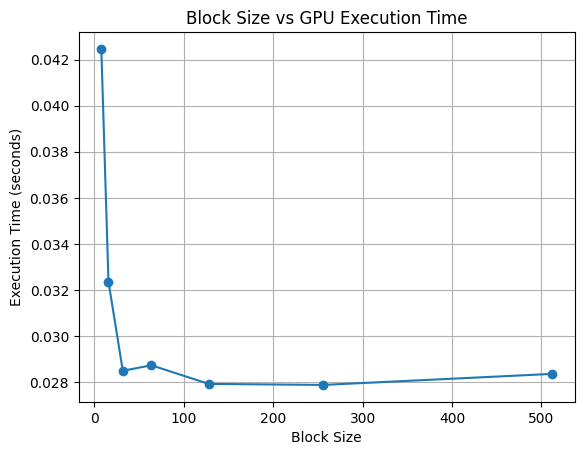
\includegraphics[width=0.8\textwidth]{block_size_time.png}
\end{center}

\end{document}
